\section{Protótipos de Tela}
\label{sec:titSecPrototipos}

Os protótipos de tela são uma versão inicial de um sistema. Eles são usados, dentre outras razões, para descobrir mais sobre um problema e suas possíveis soluções. O desenvolvimento rápido e iterativo do protótipo previne gastos desnecessários e custos controlados e os stakeholders podem fazer usos pontuais de partes do sistema desde o início do desenvolvimento \cite{Sommerville10}.
Além disso, os protótipos podem ajudar na antecipação de mudanças que podem ser requisitadas.
Para o presente projeto foram desenvolvidas três interfaces para dois tamanhos diferentes de tela, simulando um disposito de tela maior (desktop, tablet) e outro para telas menores (smartphones).

O modelo de prototipação é ideal quando o cliente não tem os requisitos muito bem definidos, que é o caso do aplicativo estudado neste documento.

Os protótipos foram desenvolvidos com o objetivo de atendender às algumas das \cite[10 Heurísticas de Nielsen]{Nielsen:1994:EEP:191666.191729}. Porém, este não é o objetivo principal para este momento.

Nas próximas subseções serão exibidos os protótipos de tela para três principais operações que o usuário poderá realizar no sistema, que são a tela que o usuário é enviado após fazer o login, a tela para criação de um novo recurso no sistema e a tela de exibição de um recurso.

\subsection{Protótipo para telas inicial do sistema}
\label{sec:titSecPrototiposHome}

\begin{figure}[H]
    \centering
    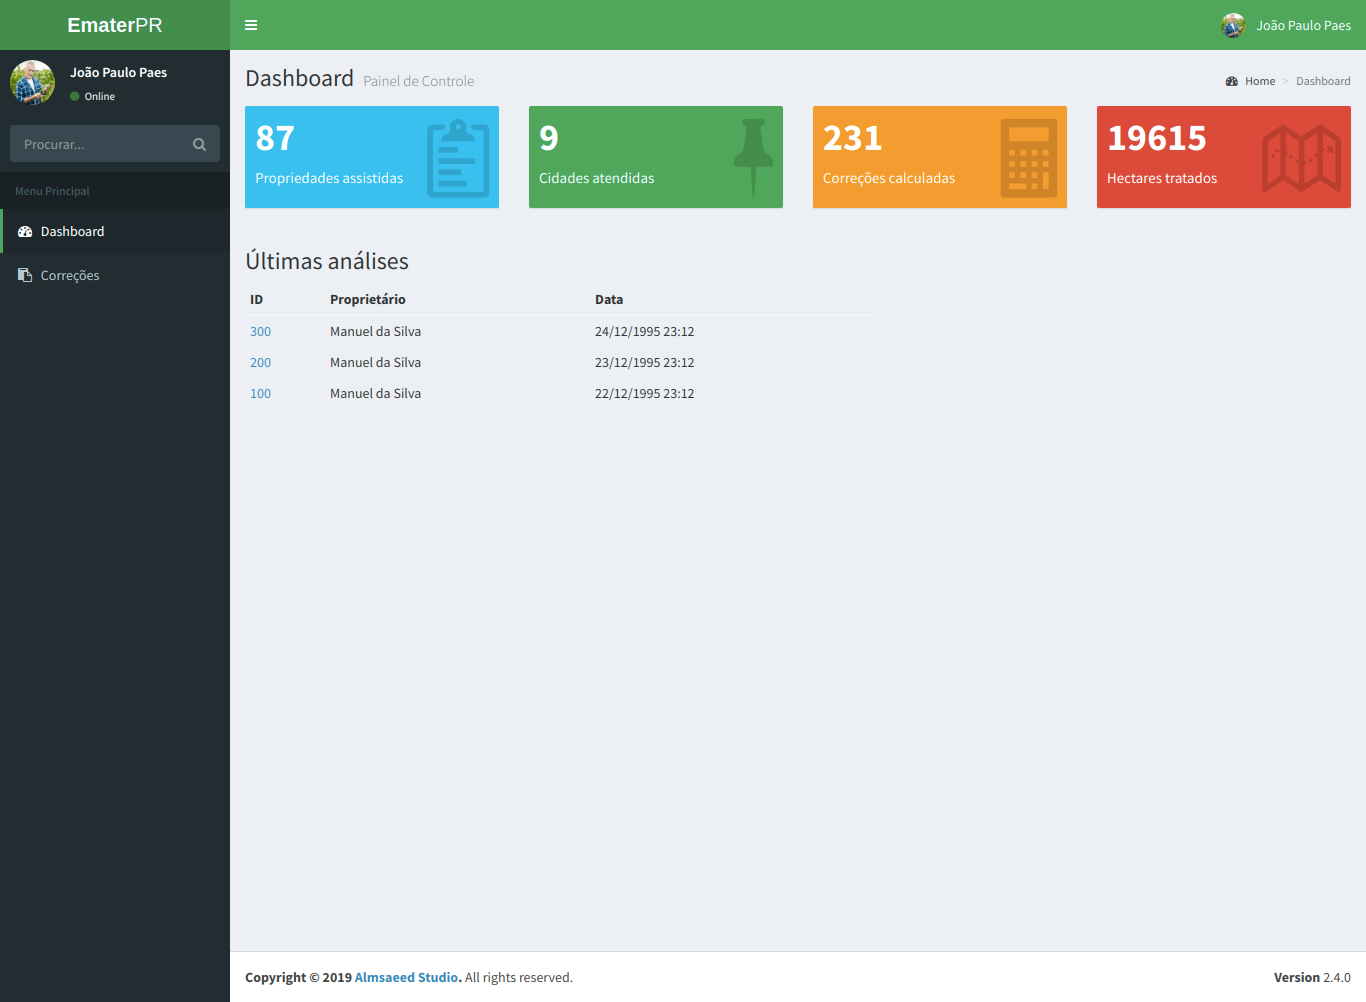
\includegraphics[width=13cm]{./dados/figuras/prototipos/home_desktop.png}
    \caption{Página que será exibida após o login do usuário na visão de um disposito desktop}
    \label{fig:prototipo_home_desk}
\end{figure}

\begin{figure}[H]
    \centering
    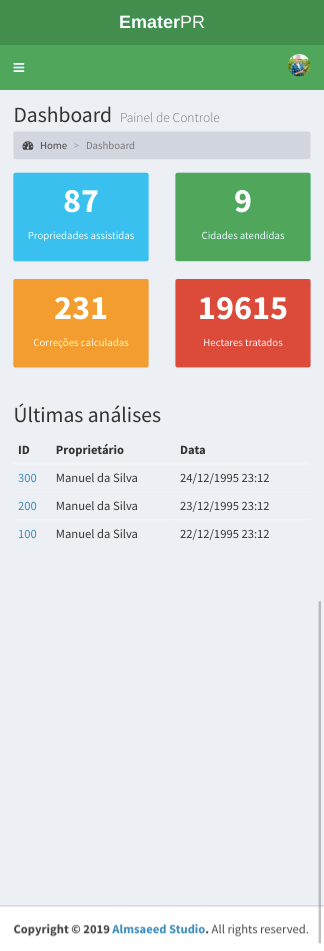
\includegraphics[width=6cm]{./dados/figuras/prototipos/home_mobile.png}
    \caption{Página que será exibida após o login do usuário na visão de um disposito mobile}
    \label{fig:prototipo_home_mobile}
\end{figure}

\subsection{Protótipo para telas de cadastro de informação}
\label{sec:titSecPrototiposCreate}

\begin{figure}[H]
    \centering
    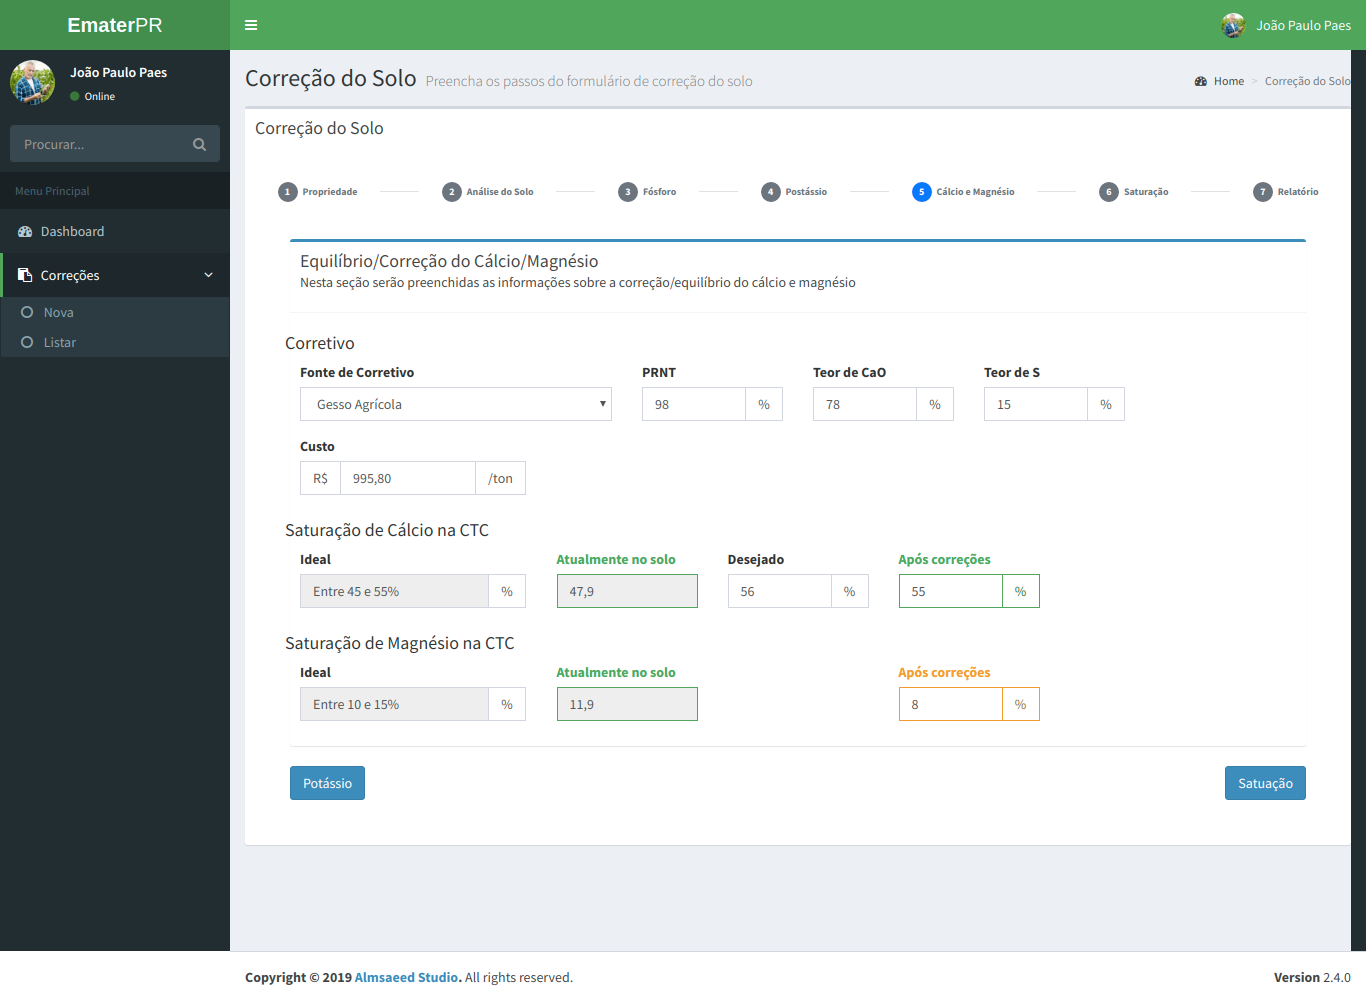
\includegraphics[width=13cm]{./dados/figuras/prototipos/create_desktop.png}
    \caption{Criação de recurso na visão de um disposito desktop}
    \label{fig:prototipo_create_desk}
\end{figure}

\begin{figure}[H]
    \centering
    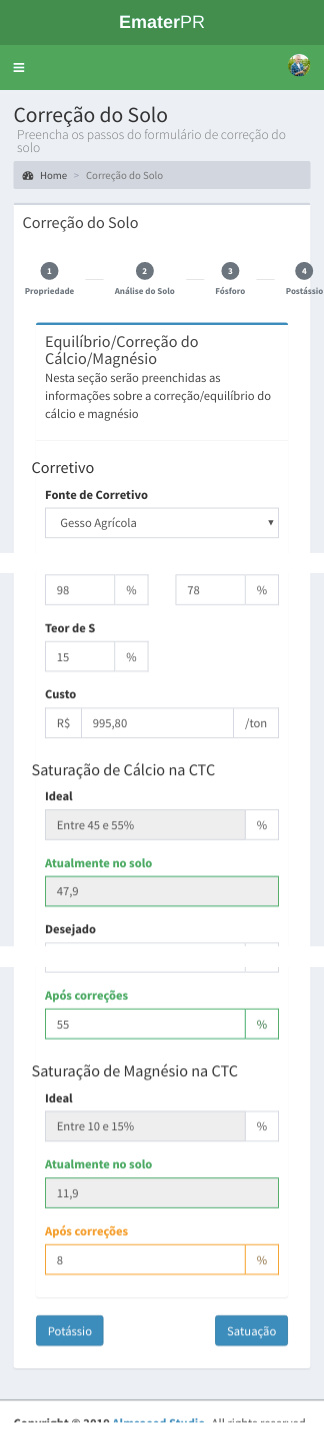
\includegraphics[width=6cm]{./dados/figuras/prototipos/create_mobile.png}
    \caption{Criação de recurso na visão de um disposito mobile}
    \label{fig:prototipo_create_mobile}
\end{figure}


\subsection{Protótipo para telas de exibição de informação}
\label{sec:titSecPrototiposShow}

\begin{figure}[H]
    \centering
    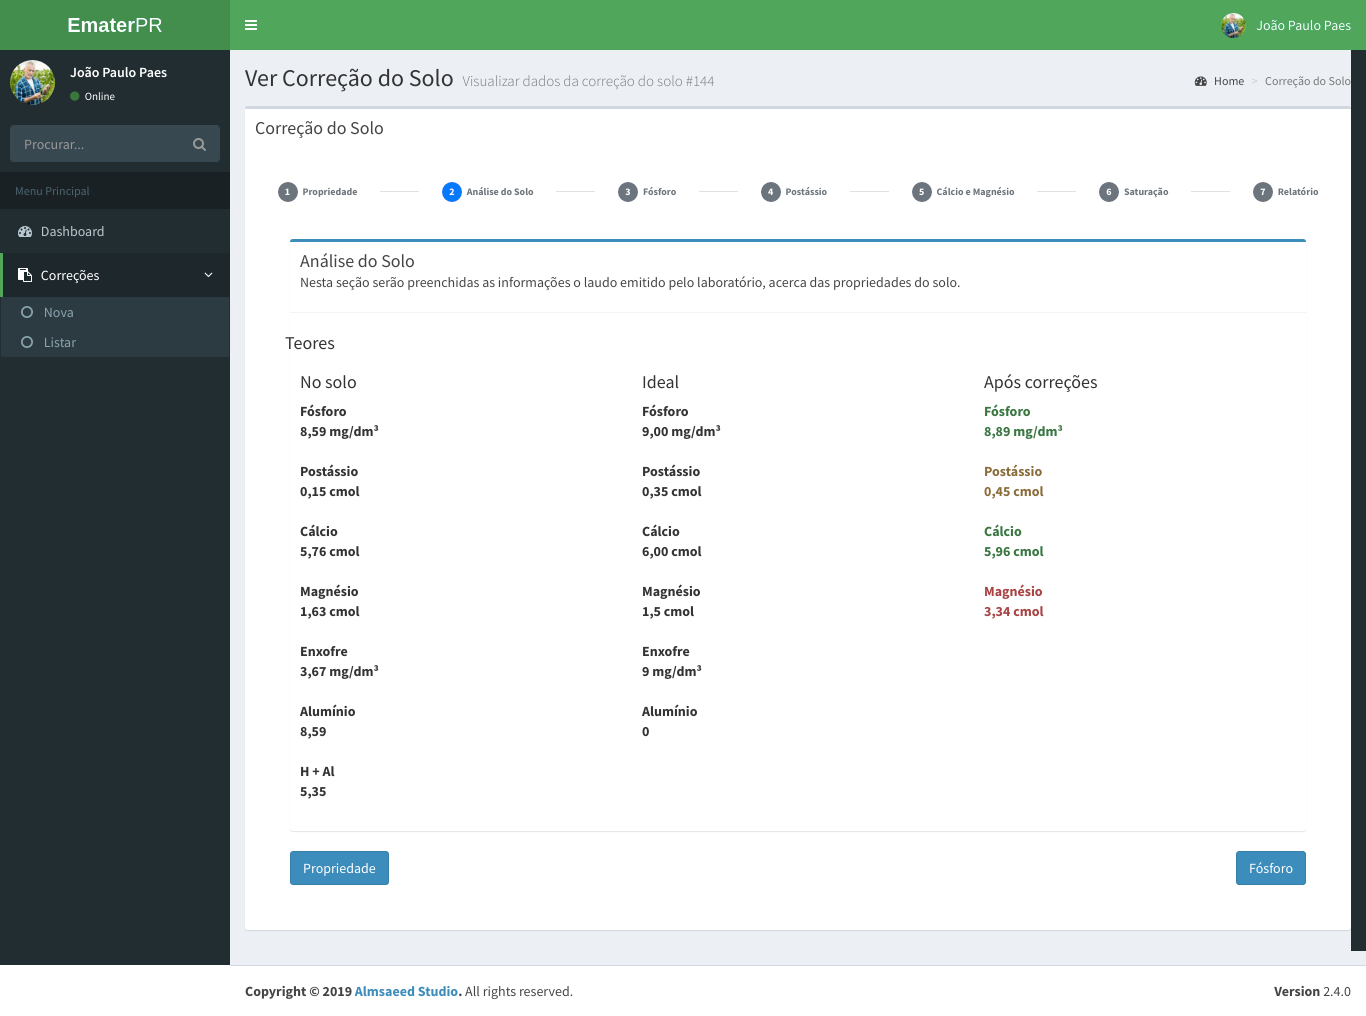
\includegraphics[width=13cm]{./dados/figuras/prototipos/show_desktop.png}
    \caption{Visualização de recurso na visão de um disposito desktop}
    \label{fig:prototipo_show_desk}
\end{figure}

\begin{figure}[H]
    \centering
    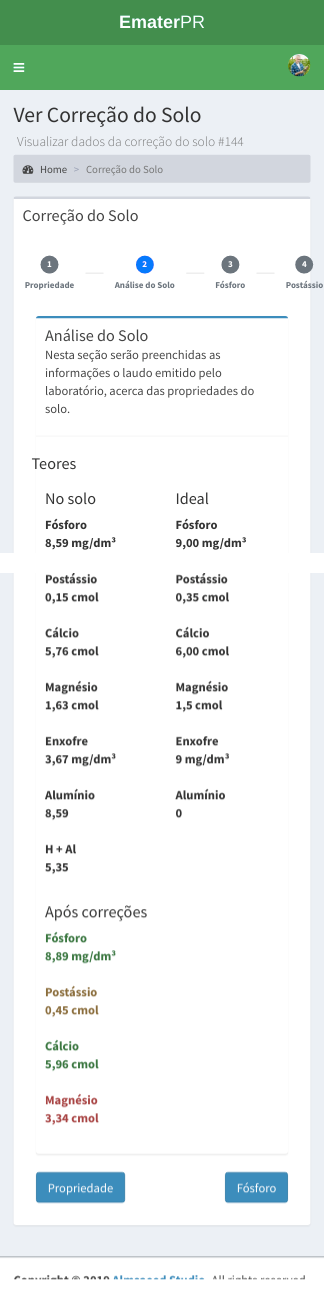
\includegraphics[width=6cm]{./dados/figuras/prototipos/show_mobile.png}
    \caption{Visualização de recurso na visão de um disposito mobile}
    \label{fig:prototipo_show_mobile}
\end{figure}